\renewcommand{\theequation}{\theenumi}
\renewcommand{\thefigure}{\theenumi}
\renewcommand{\thetable}{\theenumi}
\begin{enumerate}[label=\thesection.\arabic*.,ref=\thesection.\theenumi]
\numberwithin{equation}{enumi}
\numberwithin{figure}{enumi}
\numberwithin{table}{enumi}

\item Suppose the random varible $X$ has the following probability density function
\begin{align}
f(x)=
\begin{cases}
\alpha(x-\mu)^{\alpha-1}e^{-(x-\mu)^\alpha} &x>\mu\\
0 &x\leq\mu,
\end{cases}
\end{align}
Where $\alpha>0, -\infty<\mu<\infty$. Which of the following statements are correct? The Hazard function of $X$ is
\begin{enumerate}[label=\alph*)]
\item an increasing function for all $\alpha>0$
\item a decreasing function for all $\alpha>0$
\item an increasing function for some $\alpha>0$
\item a decreasing function for some $\alpha>0$
\end{enumerate}
%
\solution

The Hazard function of $X$,
\begin{align}
\lambda(X) = \frac{f(x)}{S(x)} \label{var/1/eq:1}
\end{align}
where $S(x)$ is the survival function given by,
\begin{align}
S(x) = P(X \geq x) = 1-F(x) = \int_{x}^{\infty}f(t)dt
\end{align}
\begin{lemma}
\begin{align}
S(x)=
\begin{cases}
e^{-(x-\mu)^\alpha} &x>\mu\\
1 &x\leq\mu
\end{cases}
\end{align}
\end{lemma}
\begin{proof}

\begin{align}
\int f(t)dt=\int \alpha(t-\mu)^{\alpha-1}e^{-(t-\mu)^\alpha}dt\\
=-e^{-(t-\mu)^\alpha} + C
\end{align}
If $x>\mu$, 
\begin{align}
S(x) = \int_{x}^{\infty} \alpha(t-\mu)^{\alpha-1}e^{-(t-\mu)^\alpha}dt\\
=-e^{-(t-\mu)^\alpha}]_{x}^{\infty}\\
=e^{-(x-\mu)^{\alpha}} \label{var/1/eq:2}
\end{align}
If $x\leq\mu$,
\begin{align}
S(x) = \int_{x}^{\mu}f(t)dt + \int_{\mu}^{\infty}f(t)dt\\
     = 0 + e^{-(\mu-\mu)^{\alpha}}\\
     =1 \label{var/1/eq:3}
\end{align}
From \eqref{var/1/eq:2} and \eqref{var/1/eq:3}, we get $S(x)$ as,
\begin{align}
S(x)=
\begin{cases}
e^{-(x-\mu)^\alpha} &x>\mu\\
1 &x\leq\mu \label{var/1/eq:4}
\end{cases}
\end{align}
\end{proof}
From \eqref{var/1/eq:1} and \eqref{var/1/eq:4}, we get
\begin{align}
\lambda(x) = 
\begin{cases}
\alpha(x-\mu)^{\alpha-1} &x>\mu\\
0 &x\leq\mu \label{var/1/eq:5}
\end{cases}
\end{align}
So,\\ if $\alpha>1$, $\lambda(x)$ is an increasing function
\begin{figure}[htp]
    \centering
    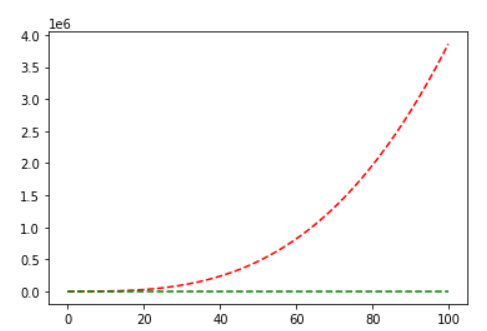
\includegraphics[width=\columnwidth]{variable/solutions/1/alphagrt1.png}
    \caption{$\alpha=2$ for red. $\alpha=1$ for green, $\mu=1$ for both}
    \label{var/1/fig:grt1}
\end{figure}
and\\ if $0<\alpha<1$, $\lambda(x)$ is a decreasing function
\begin{figure}[htp]
    \centering
    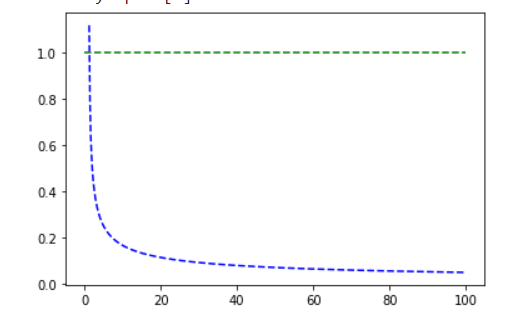
\includegraphics[width=\columnwidth]{variable/solutions/1/alphales1.png}
    \caption{$\alpha=0.5$ for blue. $\alpha=1$ for green, $\mu=1$ for both}
    \label{var/1/fig:les1}
\end{figure}
and\\ for $\alpha=1$, $\lambda(x)=1$, a constant function.\\
So, for some values of $\alpha$, it is increasing, for some it is decreasing function\\
\textbf{Therefore, answer is (C) and (D)}




\item Consider the function \textit{f(x)} defined as \textit{f(x)} = \textit{ce$^{-x^{4}}$}, $\textit{x} \in R$ . For what value of \textit{c} is \textit{f} a probability density function?\\
\begin{enumerate}
    \item $\displaystyle\frac{2}{\Gamma(1/4)}$\\\label{june/2019/52/option 1}
    \item $\displaystyle\frac{4}{\Gamma(1/4)}$\\
    \item $\displaystyle\frac{3}{\Gamma(1/3)}$\\
    \item $\displaystyle\frac{1}{4\Gamma(4)}$
\end{enumerate}
%
\solution
Consider a continuous random variable X so that the function \textit{f} can be probability density function if and only if it satisfies the condition 
\begin{align}
    \int_{-\infty}^{\infty}f_{X}(u)du = 1 \label{2019/52/equation 1}
\end{align}
Hence by applying the \eqref{2019/52/equation 1} for the function \textit{f} we get
\begin{align}
    \int_{-\infty}^{\infty}ce^{-u^{4}}du = 1\\
    2c\int_{0}^{\infty}e^{-u^{4}}du = 1\label{2019/52/equation 2}\\
    2c\int_{0}^{\infty}e^{-t}\frac{dt}{4t^{\frac{3}{4}}} = 1\\
    \frac{c}{2}\int_{0}^{\infty}e^{-t}t^{-\frac{3}{4}}dt = 1\label{2019/52/equation 3}
\end{align}
We know that gamma function for any real positive $\alpha$
\begin{align}
    \Gamma(\alpha) = \int_0^\infty x^{\alpha - 1} e^{-x} dx \label{2019/52/gammafunction}
\end{align}
Hence by using \eqref{2019/52/gammafunction} in \eqref{2019/52/equation 3} we get
\begin{align}
    \frac{c}{2}\Gamma(1/4) = 1\\
    c=\frac{2}{\Gamma(1/4)}
\end{align}
Hence $c = \displaystyle\frac{2}{\Gamma(1/4)}$ and option \eqref{2019/52/option 1} is correct.\newline\newline
The CDF of \textit{f} by using \eqref{2019/52/gammafunction} we get
\begin{align}
    F_{X}(x) &= \int_{0}^{x}f(u)du\\
             &= \frac{2}{\Gamma(\frac{1}{4})}\int_{0}^{x}e^{-u^{4}}du\\
             &= \frac{2}{4\Gamma(\frac{1}{4})}\int_{0}^{x^{4}}e^{-t}{t^{\frac{-3}{4}}}dt\\
             &= \frac{1}{2\Gamma(\frac{1}{4})}\int_{0}^{x^{4}}e^{-t}{t^{\frac{-3}{4}}}dt\\
             &= \frac{1}{2\Gamma(\frac{1}{4})}\brak{\Gamma\brak{\frac{1}{4}}-\Gamma\brak{\frac{1}{4},x^{4}}}\\
             &= \frac{1}{2\Gamma(\frac{1}{4})}\gamma\brak{\frac{1}{4},x^{4}}
\end{align}

\item Let X and Y be i.i.d random variables uniformly distributed on (0,4).Then \pr{X>Y|X<2Y} is
\begin{enumerate}
    \item 1/3
    \item 5/6
    \item 1/4
    \item 2/3
\end{enumerate}
\solution

The PDF is given by
\begin{align}
   &f_X (x)=f_Y (x)=\nonumber \begin{cases}
         \frac{1}{4}, &\text{if 0 \(< x <\) 4}\\
         0, &\text{otherwise}\\
   \end{cases} 
\end{align}    
The CDF is given by
\begin{align}
   \nonumber& F(x)=\int_{-\infty}^{x} f(x)dx \\ \nonumber
   &F_X (x)=F_Y (x)=\nonumber \begin{cases}
          0, & x\leq 0\\
         \frac{x}{4}, &\text{if 0 \(< x <\) 4}\\
          1, &x\geq4\\
   \end{cases}    
\end{align}
Using definition of conditional probability 
\begin{align}
    &\pr{X>Y|X<2Y}=\frac{\pr{Y < X< 2Y}}{\pr{X<2Y}} \label{eqn1}
\end{align}
Now finding \pr{X<2Y}
\begin{align}
    &\pr{X<2y}=F_X (2y)\\
    \implies& \pr{X<2Y}=\int_{-\infty}^{\infty} f_Y(x) \times F_X (2x)dx\\
    \implies& \pr{X<2Y}=\int_{0}^{2} \frac{x}{8}dx +\int_{2}^{4}\frac{1}{4}dx\\
    \implies& \pr{X<2Y}=\frac{3}{4}=0.75 \label{eqn2}
\end{align}
Now to find \pr{Y<X<2Y}
\begin{align}
    &\pr{y<X<2y}=F_X (2y)- F_X (y) \\
    \implies &\pr{Y<X<2Y}\\ \nonumber 
    &=\int_{-\infty}^{\infty} f_Y (x)( F_X (2x)- F_X(x))dx \\
   \implies &\int_{0}^{2}\frac{1}{4}\brak{\frac{x}{2}-\frac{x}{4}} dx +\int_{2}^{4}\frac{1}{4}\brak{1-\frac{x}{4}} dx\\
   \implies &\pr{Y<X<2Y}=\frac{1}{4}=0.25 \label{eqn3}
\end{align}
Now using \eqref{eqn1},\eqref{eqn2} and \eqref{eqn3}
\begin{align}
    \pr{X>Y|X<2Y}=\frac{1/4}{3/4}=\frac{1}{3}
\end{align}
Hence final solution is option 1) or 1/3 
%
\item Suppose $X$ is a positive random variable with the following probability density function,
\begin{align*}
f(x) = (\alpha x^{\alpha -1} + \beta x^{\beta-1} ) e^{-x^{\alpha}-x^{\beta}} ; x>0
\end{align*}
for $ \alpha >0, \beta >0$.
Then the hazard function of $X$ for some choices of $\alpha$ and $\beta$ can be
\begin{enumerate}
    \item an increasing function.
    \item a decreasing function.
    \item a constant function.
    \item a non monotonic function
\end{enumerate}
%
\solution


CDF of $X$, 
\begin{align}
    F(x) &=  \int_{-\infty}^xf(t)dt \\
    &= \int_{0}^xf(t)dt \hspace{1cm} \text{as } x>0\\
    &= \int_{-\infty}^t\left((\alpha t^{\alpha -1} + \beta t^{\beta-1} ) \times e^{-t^{\alpha}-t^{\beta}}\right)dt \\
    &= -e^{-t^{\alpha}-t^{\beta}} \Big|_0^x\\
    &= 1-e^{-x^{\alpha}-x^{\beta}}
\end{align}
Hazard function,
\begin{align}
    h(x) &= \frac{f(x)}{1-F(x)} \\
    &= \alpha x^{\alpha -1} + \beta x^{\beta-1} \\
    h^{\prime}(x) &= \alpha(\alpha -1) x^{\alpha -2} + \beta(\beta-1) x^{\beta-2}\\
     h^{\prime}(x) &= 
         \begin{cases}
    0 & \alpha=\beta=1 \\
    >0 & \text{otherwise}\\
    \end{cases}
    \end{align}
    Thus $h(x)$ can be either constant function or an increasing function.
    
    \begin{figure}[h]
    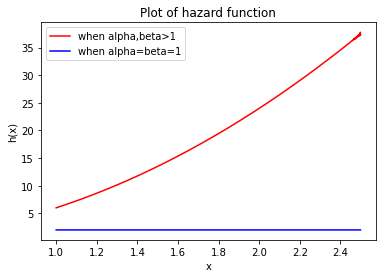
\includegraphics[width=\columnwidth]{solutions/2018/dec/118/figures/plot.png}
    \end{figure}
     From the above figure, it is verified that $h(x)$ can be either constant function or an increasing function.\\
       Correct options are 1,3.





%
\item Suppose the random variable X has the following probability density funtion 
\begin{align}
    f(x)=\begin{cases}\alpha\brak{x-\mu}^{\alpha -1}e^{-\brak{x-\mu}^\alpha};&x>\mu\\
                        0                               &x\leq\mu    
    \end{cases}\nonumber
\end{align}
where $\alpha>0,-\infty <\mu<\infty$. Which of the following are correct? The hazard function of $X$ is
\begin{enumerate}
    \item an increasing function for all $\alpha>0$
    \item a decreasing function for all $\alpha >0$
    \item an increasing function for some $\alpha>0$
    \item a decreasing function for some $\alpha>0$
\end{enumerate}
%
\solution

\newcommand{\Integral}[2]{solutions/2017/june/118/figures/\ensuremath{\int\limits_{#1}^{#2}}}
For the random variable $X$, the CDF is
\begin{align}
    F(x)&=\Integral{0}{x}f(y)dy\\
        &=\Integral{0}{\mu}0 dy +\Integral{\mu}{x}\alpha\brak{y-\mu}^{\alpha -1}e^{-\brak{y-\mu}^\alpha}\\
        &=0 -e^{-\brak{y-\mu}^\alpha}\Big|_{\mu}^{x}\\
        &=1-e^{-\brak{x-\mu}^{\alpha}}
\end{align}
For X, the hazard function $H(y)$ is defined as
\begin{align}
    H(y)&=\frac{f(y)}{1-F(y)}\nonumber\\
    \implies H(y)&=\begin{cases}\frac{\alpha\brak{y-\mu}^{\alpha -1}e^{-\brak{y-\mu}^\alpha}}{1-\brak{1-e^{-\brak{y-\mu}^{\alpha}}}};&y>\mu\\
                        0                               &y\leq\mu   
    \end{cases}\nonumber\\
    &=\begin{cases}\alpha\brak{y-\mu}^{\alpha -1};&y>\mu\\
                        0                            &y\leq\mu   
    \end{cases}\nonumber
\end{align}
Differentiating $H(y)$ w.r.t. $y$
\begin{align}
    H'(y)&=\begin{cases}\alpha\brak{\alpha - 1}\brak{y-\mu}^{\alpha -2};&y>\mu\\
                        0                            &y\leq\mu   
    \end{cases}\nonumber
\end{align}
When $y\leq \mu$ then $H'(y)$ is $0$. When $y>\mu$ then $\brak{y-\mu}^{\alpha -2}$ is positive. This implies that the sign for $H'(y)$ for $y>\mu$ is decided by the sign of $\alpha\brak{\alpha -1}$.
\begin{align}
    \alpha\brak{1-\alpha}<0
    \implies 0<\alpha<1\nonumber\\
    \alpha\brak{1-\alpha}>0\implies \alpha>1 &&\text{(ignoring $\alpha<0$)}\nonumber
\end{align}
$\therefore$ The Hazard function of $X$ is decreasing when $\alpha \in \brak{0,1}$ and increasing when $\alpha \in \brak{1,\infty}$
\vspace{0.5cm}\centering \boxed{\solution{\text{Options 3, 4}}}
% \iffalse
% \begin{figure}[h!]
%     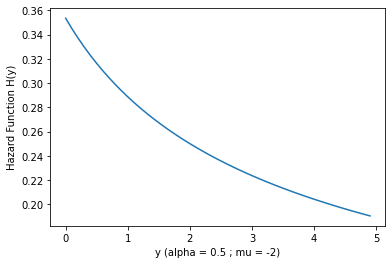
\includegraphics[width = \columnwidth]{solutions/2017/june/118/figures/Figure-1.png}
%     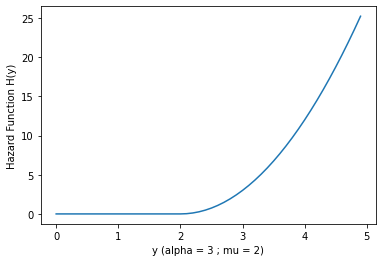
\includegraphics[width = \columnwidth]{solutions/2017/june/118/figures/Figure-2.png}
% \end{figure}
% \fi
\begin{figure}[h]
    \centering
    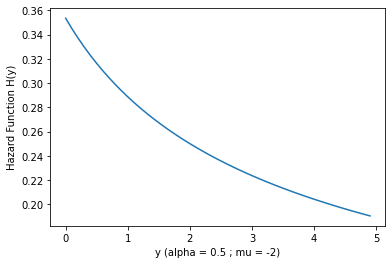
\includegraphics[width=\columnwidth-50pt]{solutions/2017/june/118/figures/Figure-1.png}
    \caption{Decreasing Hazard Function}
    \label{june/2017/118/fig:my_label1}
\end{figure}
\begin{figure}[h]
    \centering
    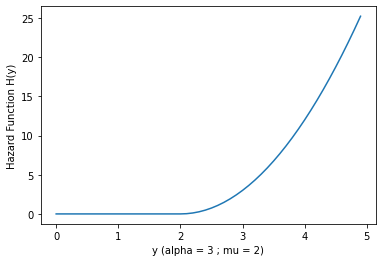
\includegraphics[width=\columnwidth-50pt]{solutions/2017/june/118/figures/Figure-2.png}
    \caption{Increasing Hazard Function}
    \label{june/2017/118/fig:my_label2}
\end{figure}

%
%
\item Let $X$ be a random variable with a certain non-degenerate distribution. Then identify the correct statements
\begin{enumerate}
    \item If $X$ has an exponential distribution then $median\brak{X}<E\brak{X}$
    \item If $X$ has a uniform distribution on an interval $[a,b]$, then $E\brak{X}<median\brak{X}$
    \item If $X$ has a Binomial distribution then $V\brak{X}<E\brak{X}$
    \item If $X$ has a normal distribution, then $E\brak{X}<V\brak{X}$
\end{enumerate}
%
\solution
Expected value\brak{E\brak{X}}:
It is nothing but weighted average
Median\brak{median\brak{X}}:
It is the value separating the higher half from the lower half of a data sample
Variance\brak{V\brak{X}}:
It is the expectation of the squared deviation of a random variable from its mean
\begin{enumerate}
    \item Let's consider $X$ has an exponential distribution.
    \begin{align}
        X \sim Exp\brak{\lambda}
    \end{align}
    where $\lambda$ is rate parameter.
    
    Probability function of exponential distribution,
    \begin{align}
        f_X\brak{x}=
        \begin{cases}
            \lambda e^{-\lambda x} & x\geq0\\
            0 & x<0
        \end{cases}
    \end{align}
    The expected value of $X \sim Exp\brak{\lambda}$,
    \begin{align}
        E\brak{X}=\frac{1}{\lambda}
    \end{align}
    The median of $X \sim Exp\brak{\lambda}$,
    \begin{align}
        median\brak{X}=\frac{\ln{2}}{\lambda}
    \end{align}
    \begin{align}
        \ln{2}<1\\
        \frac{\ln{2}}{\lambda}<\frac{1}{\lambda}\\
         median\brak{X}<E\brak{X}
    \end{align}
    Hence, option $1$ is correct.
    
    \item Let's consider $X$ has a uniform distribution in interval $[a,b]$,
    \begin{align}
        X \sim U\brak{a,b}
    \end{align}
    where,
    $a=$ lower limit
    
    $b=$ upper limit
    
    Probability function of uniform distribution,
    \begin{align}
        f_X\brak{k}=
        \begin{cases}
            \frac{1}{b-a} & a\leq x\leq b\\
            0 & x < a, x > b
        \end{cases}
    \end{align}
    The expected value of $X \sim U\brak{a,b}$,
    \begin{align}
        E\brak{X}=\frac{1}{2}\brak{a+b}
    \end{align}
    The median of $X \sim U\brak{a,b}$,
    \begin{align}
        median\brak{X}=\frac{1}{2}\brak{a+b}
    \end{align}
    \begin{align}
        E\brak{X}=median\brak{X}
    \end{align}
    Hence, option $2$ is incorrect.
    
    \item Let's consider $X$ has a binomial distribution,
    \begin{align}
        X \sim B\brak{n,p}
    \end{align}
    where,
    $n=$ no. of trails
    
    $p=$ success parameter
    
    Probability function of binomial distribution,
    \begin{align}
        f_X\brak{k}=
        \begin{cases}
            {^n C_k}p^k(1-p)^{n-k} & 0\leq k\leq n\\
            0 & otherwise
        \end{cases}
    \end{align}
    The expected value of $X \sim B\brak{n,p}$,
    \begin{align}
        E\brak{X}=np
    \end{align}
    The variance of $X \sim B\brak{n,p}$,
    \begin{align}
        V\brak{X}=\sigma^2=n p(1-p)
    \end{align}
    \begin{align}
        1-p\leq1\\
        n p(1-p)\leq n p\\
        V\brak{X}\leq E\brak{X}
    \end{align}
    Hence, option $3$ is incorrect.
    
    \item Let's consider $X$ has a normal distribution,
    \begin{align}
        X \sim N\brak{\mu,\sigma^2}
    \end{align}
    where,
    $\mu=$ mean of distribution
    
    $\sigma^2=$ variance
    
    Probability function of normal distribution,
    \begin{align}
        f_X\brak{k}=\frac{1}{\sigma\sqrt{2\pi}}e^{-\brak{\frac{x-\mu}{2\sigma}}^2}
    \end{align}
    The expected value of $X \sim N\brak{\mu,\sigma^2}$,
    \begin{align}
        E\brak{X}=\mu
    \end{align}
    The variance of $X \sim N\brak{\mu,\sigma^2}$,
    \begin{align}
        V\brak{X}=\sigma^2
    \end{align}
    $E\brak{X}$ and $V\brak{X}$ are user defined. So, they can take any value.
    
    Hence, option $4$ is incorrect.
    \end{enumerate}
    
%
\item A fair coin is tossed repeatedly. Let $X$ be the number of tails before the first heads occurs. Let $Y$ denote the number of tails between the first and second heads. Let $X+Y = N$. Then which of the following are true?
\begin{enumerate}
    \item X and Y are independent random variables with
    {\footnotesize
    \begin{align}
        \pr{X = k} = \pr{Y = k} =
        \begin{cases}
            2^{-(k+1)} & k=0,1,2 \ldots
            \\
            0 & otherwise
        \end{cases}
    \end{align}
    }
    \item $N$ has a probability mass function given by
    {\small
     \begin{align}
        \pr{N = k} =
        \begin{cases}
            (k-1)2^{-k} & k=2,3,4 \ldots
            \\
            0 & otherwise
        \end{cases}
    \end{align}
    }
    \item Given $N = n$, the conditional distribution of X and Y are independent
    \item Given $N = n$
     \begin{align}
        \pr{X = k} =
        \begin{cases}
            \frac{1}{n+1} & n=0,1,2 \ldots
            \\
            0 & otherwise
        \end{cases}
    \end{align}
\end{enumerate}
%

\item Assume that $X\sim Binomial(n, p)$ for some $n\geq 1$ and $0<p<1$
and $Y\sim poisson(\lambda)$for some $\lambda > 0$.Suppose E[X]=E[Y].Then
\begin{enumerate}
    \item $var(X)=Var(Y)$\\
    \item $var(X)<Var(Y)$\\
    \item $var(Y)<Var(X)$\\
    \item $Var(X)$ may be larger or smaller than $Var(Y)$ depending on the values of n,p and $\lambda$
\end{enumerate}
%
%
\solution
For the random variable $$X\sim Binomial(n, p)$$
As we know,
\begin{align}
E[X]&=np\\
Var(X)&=np(1-p) \label{june/2015/53a}
\end{align}
for the random variable $$Y\sim poisson(\lambda)$$
As we know,
\begin{align}
E[Y]&=\lambda\\
Var(Y)&=\lambda \label{june/2015/53b}
\end{align}
given that,
\begin{align}
E[X]&=E[Y]\\
np&=\lambda \label{june/2015/53c}
\end{align}
from \eqref{june/2015/53a},
\begin{align}
Var(X)&=np(1-p)
\end{align}
using \eqref{june/2015/53c},
\begin{align}
Var(X)&=\lambda(1-p)
\end{align}
\begin{table}[ht]
\caption{Mean and Variance for random variables X and Y}
\begin{center}
    \begin{tabular}{|c|c|c|}
    \hline
     & $X$&$Y$\\
    \hline
    E& $\lambda$& $\lambda$\\
    \hline
     $var$& $\lambda(1-p)$ & $\lambda$\\
    \hline
    \end{tabular}
\end{center} 
\label{june/2015/53tab:1}
\end{table}
using \eqref{june/2015/53b},
\begin{align}
Var(X)&=Var(Y)(1-p)\\
\frac{Var(X)}{Var(Y)}&= 1-p
\end{align}
as,
\begin{align}
1-p &<1\\
\frac{Var(X)}{Var(Y)}&<1\\
Var(X) &< Var(Y)
\end{align}
$\therefore$ $Var(Y) >Var(X)$, independent of n,p and $\lambda$.
\begin{enumerate}
    \item $var(X)=Var(Y)$\\
          using TABLE \ref{june/2015/53tab:1},
          \begin{align}
          \lambda(1-p) = \lambda\\
          1-p=1\\
          p=0
          \end{align}
          which is wrong as per the question$(0<p<1)$.
          hence the option is incorrect.
    \item $var(X)<Var(Y)$\\
          using TABLE \ref{june/2015/53tab:1},
          \begin{align}
          \lambda(1-p) < \lambda\\
          1-p<1\\
          p>0
          \end{align}
          which is true as per the question$(0<p<1)$.
          hence the option is correct.
    \item $var(Y)<Var(X)$\\
     using TABLE \ref{june/2015/53tab:1},
          \begin{align}
          \lambda(1-p) > \lambda\\
          1-p>1\\
          p<0
          \end{align}
          which is wrong as per the question$(0<p<1)$.
          hence the option is incorrect.
    \item $Var(X)$ may be larger or smaller than $Var(Y)$ depending on the values of n,p and $\lambda$.\\
    Wrong, since we have shown that irrespective of the values of lambda, n, and p, $var(y) > var(x)$
\end{enumerate}

%
%
\item Let $X$ be a non-negative integer valued random variable with probability mass function $f(x)$ satisfying $(x+1)f(x+1)=(\alpha + \beta x)f(x)$, $x=0,1,2,...$; $\beta \neq 1$. You may assume that $E(X)$ and $Var(X)$ exist. Then which of the following statements are true?

\begin{enumerate}
    \item $E(X)=\dfrac{\alpha}{1-\beta}$ \vspace{0.2cm}
    \item $E(X)=\dfrac{\alpha^2}{(1-\beta)(1+\alpha)}$ \vspace{0.2cm}
    \item $Var(X)=\dfrac{\alpha^2}{(1-\beta)^2}$ \vspace{0.2cm}
    \item $Var(X)=\dfrac{\alpha}{(1-\beta)^2}$
\end{enumerate}
%
\solution
For a discrete random variable $X$ with P.D.F. $f(x)$ and which can take values from a set $\mathbb{S}$,
\begin{align} \label{june2013-75:eq-1}
    E(X)= \sum_{x \in \mathbb{S}}xf(x)
\end{align}
And,
\begin{align} \label{june2013-75:eq-2}
    E(X^2) =\sum_{x \in \mathbb{S}}x^2f(x)
\end{align}
Also, as $f(x)$ is the P.D.F.,
\begin{align} \label{june2013-75:eq-3}
    \sum_{x \in \mathbb{S}}f(x) = 1
\end{align}
Given, for $x \in \mathbb{S}=\{0,1,2,...n\}$,
\begin{align} \label{june2013-75:eq-4}
    (x+1)f(x+1)=(\alpha + \beta x)f(x)
\end{align}
Summing both sides for $x \in \mathbb{S}$ we get,
\begin{align}
    \sum_{x=0}^n(x+1)f(x+1)=\sum_{x=0}^n(\alpha +\beta x)f(x)
\end{align}
Replacing $x+1$ with $x$ in L.H.S. we get, 
\begin{align}
    \sum_{x=1}^{n+1}xf(x)=\sum_{x=0}^n(\alpha +\beta x)f(x)
\end{align}
Rewriting LHS, we get,
\begin{align}
    \sum_{x=0}^nxf(x)+(n+1)f(n+1)=\sum_{x=0}^n(\alpha +\beta x)f(x)
\end{align}
But as $x \in \{0,1,2...n\}$, $f(n+1)=0$. So the equation becomes
\begin{align}
    \sum_{x=0}^nxf(x)=\alpha \sum_{x=0}^nf(x) + \beta \sum_{x=0}^nxf(x)
\end{align}
Using \eqref{june2013-75:eq-1} and \eqref{june2013-75:eq-3}, we get,
\begin{align} 
    E(X)=\alpha(1) + \beta E(X)
\end{align}
So,
\begin{align} \label{june2013-75:eq-5}
    E(X)=\dfrac{\alpha}{1-\beta}
\end{align}
Now in \eqref{june2013-75:eq-4}, multiplying both sides by $(x+1)$, we get,
\begin{align}
    (x+1)^2f(x+1)=(\alpha + \beta x)(x+1)f(x)
\end{align}
Summing both sides for $x \in \mathbb{S}$ we get,
\begin{align}
    \sum_{x=0}^n(x+1)^2f(x+1)=\sum_{x=0}^n(\alpha +\beta x)(x+1)f(x)
\end{align}
Replacing $x+1$ with $x$ in L.H.S. we get, 
\begin{align}
    \sum_{x=1}^{n+1}x^2f(x)=\sum_{x=0}^n(\beta x^2f(x) + (\alpha+\beta)xf(x) + \alpha f(x))
\end{align}
Rewriting LHS similarly as before, we get,
\begin{align}
    \sum_{x=0}^nx^2f(x)=\beta \sum_{x=0}^nx^2f(x) + \nonumber \\
    (\alpha + \beta)\sum_{x=0}^nxf(x) + \alpha \sum_{x=0}^nf(x)
\end{align}
Using \eqref{june2013-75:eq-1}, \eqref{june2013-75:eq-2} and \eqref{june2013-75:eq-3}, we get,
\begin{align}
    E(X^2)=\beta E(X^2) + (\alpha + \beta)E(X) + \alpha (1) 
\end{align}
Using \eqref{june2013-75:eq-5}
\begin{align}
    E(X^2)(1-\beta)=\dfrac{\alpha(\alpha+\beta)}{1-\beta} + \alpha
\end{align}
So,
\begin{align} \label{june2013-75:eq-6}
    E(X^2)=\dfrac{\alpha^2+\alpha}{(1-\beta)^2}
\end{align}
Now,
\begin{align}
    Var(X)=E(X^2)-(E(X))^2
\end{align}
Using \eqref{june2013-75:eq-5} and \eqref{june2013-75:eq-6},
\begin{align}
    Var(X)=\dfrac{\alpha^2+\alpha}{(1-\beta)^2}-\dfrac{\alpha^2}{(1-\beta)^2}
\end{align}
So,
\begin{align}
    Var(X)=\dfrac{\alpha}{(1-\beta)^2}
\end{align}
So, options 1 and 4 are correct.
%
\item Let X be a random variable with probability density function,
\begin{align}
    f(x)=\alpha(x-\mu)^{\alpha-1}e^{-(x-\mu)^{\alpha}}
\end{align}
such that $-\infty<\mu<\infty\;;\alpha>0\;;x>\mu$, The hazard function is: 
\begin{enumerate}
    \item constant for all $\alpha$
    \item an increasing function for some $\alpha$
    \item independent of $\alpha$
    \item independent of $\mu$ when $\alpha=1$
\end{enumerate}
%
\solution
Given PDF of X,
\begin{align}
    f(x)=\alpha(x-\mu)^{\alpha-1}e^{-(x-\mu)^{\alpha}}\label{june2014-71:3}
\end{align}
\textbf{Important property}(using in \eqref{june2014-71:1} as $x>\mu$):
Given $x-y>0$ and $-\infty<y<\infty$, then
\begin{align}
    \lim_{x \to -\infty} x-y=0
\end{align}
CDF of X,
\begin{align}
    F(x)&=\int_{-\infty}^x{f(x)\;dx}\\
    &=\int_{-\infty}^x{\alpha(x-\mu)^{\alpha-1}e^{-(x-\mu)^{\alpha}}dx}\\
    &=\int_{-\infty}^x{e^{-(x-\mu)^{\alpha}}d(x-\mu)^{\alpha}}\\
    &=\sbrak{\frac{e^{-(x-\mu)^{\alpha}}}{-1}}_{-\infty}^x\\
    &=-e^{-(x-\mu)^{\alpha}}-\lim_{x \to -\infty} \frac{e^{-(x-\mu)^{\alpha}}}{-1}\label{june2014-71:1}\\
    &=-e^{-(x-\mu)^{\alpha}}+ {e^{-(0)^{\alpha}}}\\
   F(x) &=1-e^{-(x-\mu)^{\alpha}}\label{june2014-71:2}
\end{align}
Hazard function $\beta(x)$,(using \eqref{june2014-71:3} and \eqref{june2014-71:2})
\begin{align}
    \beta(x)&=\frac{f(x)}{1-F(x)}\\
    &=\frac{\alpha(x-\mu)^{\alpha-1}e^{-(x-\mu)^{\alpha}}}{1-(1-e^{-(x-\mu)^{\alpha}})}\\
    &=\frac{\alpha(x-\mu)^{\alpha-1}e^{-(x-\mu)^{\alpha}}}{e^{-(x-\mu)^{\alpha}}}\\
    \beta(x)&=\alpha(x-\mu)^{\alpha-1}
\end{align}
\begin{enumerate}
    \item $\beta(x)$ is not constant for all $\alpha$
    \item $\beta(x)=\alpha(x-\mu)^{\alpha-1}$ is an increasing function for $\alpha<0 \;or\; \alpha>1$ as given $x-\mu>0$ for all x.
    
    \textbf{Proof: }
    Using first derivative test, A function is increasing iff its first derivative is positive for all x. 
    \begin{align}
        \dfrac{d}{dx} \beta(x)&=  \dfrac{d}{dx} \alpha(x-\mu)^{\alpha-1}\\
        &= \alpha(\alpha-1)(x-\mu)^{\alpha-2}\label{june2014-71:0}
    \end{align}
    For \eqref{june2014-71:0} to be positive, (As given $x-\mu>0$)
    \begin{align}
        \alpha(\alpha-1)(x-\mu)^{\alpha-2}&>0\\
        \alpha(\alpha-1)&>0\\
        \implies \alpha \in \brak{-\infty,0}\cup \brak{1,\infty}
    \end{align}
    $\therefore \beta(x)$ an increasing function for some $\alpha$
    \item $\beta(x)$ is dependent of $\alpha$
    \item when $\alpha=1$,
\begin{align}
    \beta(x)&=\alpha(x-\mu)^{0}=\alpha
\end{align}
Therefore the hazard function is independent of $\mu$ when $\alpha=1$.
\end{enumerate}
\textbf{ANSWER: (2) and (4)}
%
\item 
A point is chosen at random from a circular disc shown below. What is the probability that the point lies in the sector OAB?\\

\begin{tikzpicture}
\draw (0,0) circle (3cm);
\draw (0,0) node{O}-- (2,2.25) node{A};
\draw (0,0) -- (2.828,1) node{B};
\end{tikzpicture}\\

( where $\angle$AOB = x radians )


    \begin{enumerate}
        \item $\frac{2x}{\pi}$
        \item $\frac{x}{\pi}$
        \item $\frac{x}{2\pi}$
        \item $\frac{x}{4\pi}$
    \end{enumerate}

%
\solution
\section*{\textbf{solution}}
Let $X \in \{0,1\}$ be a random variable such that X=0 means we choose a point lying in sector OAB and X=1 means that we choose a point lying outside sector OAB and inside the circle.\\

Area of a sector subtending an angle $\theta$ at the centre of circle with radius a is given by :
\begin{equation}
    A = \frac{1}{2}a^2\theta
\end{equation}
where $\theta$ is in radians.\\

Let the radius of circle shown in figure be r. It is given that  sector  OAB subtends an angle of x radians at the centre of the circle.\\

Probability that the chosen point lies in sector OAB is:
\begin{align}
    \pr{X=0} =& \frac{\text{Area of sector OAB}}{\text{Area of circle}}\\
       =& \frac{\frac{1}{2} r^2 x}{\pi r^2}\\
       =& \frac{x}{2\pi}
\end{align}

$\therefore$The correct answer is \textbf{option (3)} $\frac{x}{2\pi}$.

\section*{\textbf{alternate solution}}
The joint pdf is given by:
\begin{equation}
 \texorpdfstring{f\textsubscript{r$\theta$}}{f r $\theta$}(r,\theta)= \begin{cases}
                        \dfrac{r}{\pi R^2}  & \text{if 0 $<$ r $<$ R , 0 $<$ $\theta$ $<$ 2$\pi$ }\\
                        0  & \text{otherwise}
                        \end{cases}
\end{equation}

Let A $\equiv$ (R,  $\theta _2$) and B $\equiv$ (R,  $\theta _1$). \\
Hence,
\begin{equation}
(\theta _2 - \theta _1)= x    
\end{equation}

We want $\theta$ $\in$ ($\theta _1$ , $\theta _2$) and r $\in$ (0,R) for point to lie in the sector.
Let the point to be chosen be (r, $\theta$).\\

So, Required probability is:
\begin{align}
 \nonumber  \pr{\theta_1<\theta<\theta_2 , 0<r<R}\\
    =& \Int_{\theta_1}^{\theta_2} \Int_{0}^{R} \dfrac{r}{\pi R^2} \,dr\,d\theta \\
    =& \Int_{\theta_1}^{\theta_2} \dfrac{1}{\pi R^2} \dfrac{r^2}{2} \Bigg|_0^R \\
    =& \Int_{\theta_1}^{\theta_2} \dfrac{R^2}{2\pi R^2} \,d\theta  \displaybreak  \\
    =& \Int_{\theta_1}^{\theta_2} \dfrac{1}{2\pi} \,d\theta\\
    =& \dfrac{\theta}{2\pi} \Bigg|_{\theta_1}^{\theta_2} \\
    =& \dfrac{\theta_2 - \theta_1}{2\pi} \\
    =& \dfrac{x}{2\pi}
\end{align}
    
$\therefore$The correct answer is \textbf{option (3)} \Large $\frac{x}{2\pi}$.


%
\item Let $X$ and $Y$ be independent random variables each following a uniform distribution on $(0,1)$.Let $W=XI_{\{Y\leq X^2\}}$,where $I_A$ denotes the indicator function of set $A$.Then which of the following statements are true? \\
\begin{enumerate}
\item The cumulative distribution function of $W$ is given by
\begin{align}
  F_W(t)=t^2I_{\{0\leq t \leq 1\}}+ I_{\{t > 1\}}
\end{align}
\item $P\sbrak{W>0}=\frac{1}{3}$
\item The cumulative distribution function of $W$ is continuous
\item The cumulative distribution function of $W$ is given by
\begin{align}
  F_W(t)=\brak{\frac{2+t^3}{3}}I_{\{0\leq t \leq 1\}}+ I_{\{t > 1\}}
\end{align}
\end{enumerate}
%
\solution






Given $X$ and $Y$ are two independent random\\
variables. \\
Given $W=XI_{\{Y\leq X^2\}}$ \\
$X \in \brak{0,1}$ , $Y \in \brak{0,1}$ , $W \in [0,1)$\\
\begin{enumerate}
\item We need to find CDF of $W$
\begin{enumerate}
\item The PDF for $X$ is
\begin{align}
p_X(x) = 
\begin{cases}
     1 & 0 < x  < 1 \\
     0 & otherwise 
\end{cases}\label{june2013-70:1}
\end{align}
\item The CDF for $X$ is
\begin{align}
F_{X}(x)  = 
\begin{cases}
      0 & x \leq 0 \\
      x & 0 < x < 1 \\
      1 & otherwise
\end{cases}  \label{june2013-70:eq:2}
\end{align}
\item The PDF for $Y$ is
\begin{align}
p_{Y}(y)  = 
\begin{cases}
      1 & 0 < y < 1 \\
      0 & otherwise 
\end{cases} \label{june2013-70:3}
\end{align}
\item The CDF for $Y$ is
\begin{align}
F_{Y}(y)  = 
\begin{cases}
      0 & y \leq 0 \\
      y & 0 < y < 1 \\
      1 & otherwise 
\end{cases}\label{june2013-70:4}
\end{align}
\item $I_{\{Y\leq X^2\}}$ is defined as follows
\begin{align} 
I_{\{Y\leq X^2\}} =
\begin{cases}
    1 & y \leq x^2  \\
    0 & otherwise 
\end{cases} \label{june2013-70:5}
\end{align}
\item $W$ is defined as follows
\begin{align}
W  = 
\begin{cases}
    x & y \leq x^2 \\
    0 & otherwise
\end{cases}  \label{june2013-70:6}
\end{align}
From \eqref{june2013-70:6}
\begin{align}
p_W(W=0) &= \Pr(I_{\{Y\leq X^2\}}=0) \\
         &=\Pr(x^2 <y) \label{june2013-70:7}
\end{align}
\item Let $Z=X^2-Y$ be a random variable where $Z \in \brak{-1,1}$

\begin{align}
F_{X^2}(u)&=\Pr(X^2 \leq u) \\
          &=\Pr(X \leq \sqrt{u}) \\
          &=F_X(\sqrt{u}) \label{june2013-70:8}
\end{align}
\begin{enumerate}
\item From \eqref{june2013-70:eq:2},The CDF for $X^2$ is
\begin{align}
F_{X^2}(u)  = 
\begin{cases}
      0 & u \leq 0 \\
      \sqrt{u} & 0 < u < 1 \\
      1 & otherwise
\end{cases} \label{june2013-70:9}
\end{align}
\item The PDF for $X^2$ is
\begin{align}
p_{X^2}(u)  = 
\begin{cases}
      \frac{1}{2\sqrt{u}} & 0 < u < 1 \\
      0 & otherwise
\end{cases} \label{june2013-70:10}
\end{align}
\begin{align}
F_{\{-Y\}}(v)&=\Pr(-Y \leq v) \\
          &=\Pr(Y \geq -v) \\
          &=1-F_Y(-v) \label{june2013-70:11}
\end{align}
\item From \eqref{june2013-70:4},The CDF for $(-Y)$ is
\begin{align}
F_{\{-Y\}}(v)  = 
\begin{cases}
      0 & v \leq -1\\
      1+v & -1 < v < 0 \\
      1 & otherwise 
\end{cases}\label{june2013-70:12}
\end{align}
\item The PDF for $(-Y)$ is
\begin{align}
p_{\{-Y\}}(v)  = 
\begin{cases}
      1 & -1 < v < 0 \\
      0 & otherwise
\end{cases} \label{june2013-70:p-y}
\end{align}
\item $Z=X^2-Y$ $\implies  z=u+v$\\
Using convolution
\begin{align}
p_Z(z)=\int_{- \infty}^{\infty} p_{X^2}(z-v)p_{\{-Y\}}(v) \mathrm{dv} \label{june2013-70:pz}
\end{align}
Solving \eqref{june2013-70:pz} using \eqref{june2013-70:p-y},\eqref{june2013-70:10} for $z \in (-1,1)$, we get PDF of $Z$ as follows
\begin{align}
p_{Z}(z)  = 
\begin{cases}
      \sqrt{z+1} & -1 < z \leq 0 \\
      1-\sqrt{z} & 0 < z <1 \\
      0 & otherwise 
\end{cases} \label{june2013-70:13}
\end{align}
\item CDF of $Z$ as follows
\begin{align}
F_{Z}(z)  = 
\begin{cases}
      \frac{2}{3}{(z+1)}^\frac{3}{2} & -1 < z \leq 0 \\
      z-\frac{2}{3}{z}^\frac{3}{2} & 0 < z < 1 \\
      1 & otherwise
\end{cases} \label{june2013-70:14}
\end{align}

\end{enumerate}

\item using \eqref{june2013-70:14} to find $p_W(W=0)$
\begin{align}
p_W(W=0) &=\Pr(x^2 <y) \\
         &=F_z(0) \\
         &=\frac{2}{3} \label{june2013-70:15}
\end{align}

\item $W=t \implies X=t $ where $t \in (0,1)$
\begin{align}
p_{W}(t) = \int_{- \infty}^{\infty} p_X(t)I_{\{y\leq t^2\}} \mathrm{dy}
\end{align}
\begin{align}
   0 &< y < 1 \label{june2013-70:16} \\
   0 &< y \leq t^2  \label{june2013-70:17}
\end{align}
For $ 0 < t < 1 $,
\begin{align}
p_W(t) &= \int_{0}^{t^2} p_X(t)I_{\{y\leq t^2\}} \mathrm{dy} \\
       &= t^2 \label{june2013-70:18}
\end{align}
\item $\therefore$ PDF of $W$ is as follows
\begin{align}
p_{W}(t)  = 
\begin{cases}
  \frac{2}{3}& t=0 \\
  t^2 & 0 < t < 1 \\
  0 & otherwise
\end{cases} \label{june2013-70:19}
\end{align}
\item The CDF  of $W$ is as follows:
\begin{align}
F_W(t)  = 
\begin{cases}
  0 & t<0 \\
  \frac{2+t^3}{3}& 0 \leq t\leq 1\\
  1 & otherwise
\end{cases} \label{june2013-70:20}
\end{align}
\end{enumerate}
\item We need to find $P\sbrak{W>0}$
\begin{align}
\Pr(W > 0)&= 1- F_W(0) \\
           &=\frac{1}{3} \label{june2013-70:21} \\
\therefore \Pr(W>0)&=\frac{1}{3}
\end{align}
\item CDF of $W$ is discontinuous at $W=0$.\\
$\therefore$ option $3$ is incorrect.\\
\item The CDF in \eqref{june2013-70:20} can be written as
\begin{align}
  F_W(t)=\brak{\frac{2+t^3}{3}}I_{\{0\leq t \leq 1\}}+ I_{\{t > 1\}}
\end{align}
$\therefore$ option $2$ and $4$ are correct.
\begin{figure}[htb!]
\begin{center}
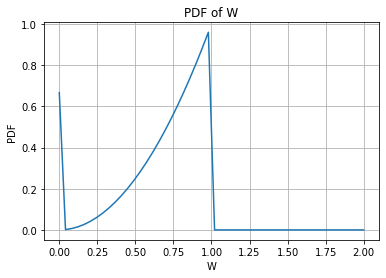
\includegraphics[width=\columnwidth]{solutions/2013/june/70/figures/assignment8pdf.png}
\end{center}
\end{figure}

\begin{figure}[htb!]
\begin{center}
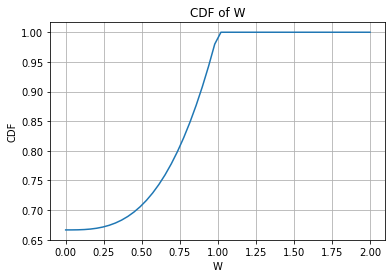
\includegraphics[width=\columnwidth]{solutions/2013/june/70/figures/assignment8cdf.png}
\end{center}
\end{figure}
\end{enumerate}

%
%
\newcommand{\tikzAngleOfLine}{\tikz@AngleOfLine}
  \def\tikz@AngleOfLine(#1)(#2)#3{%
  \pgfmathanglebetweenpoints{%
    \pgfpointanchor{#1}{center}}{%
    \pgfpointanchor{#2}{center}}
  \pgfmathsetmacro{#3}{\pgfmathresult}%
  }

\item A point is chosen at random from a circular disc shown below. What is the probability that the point lies in the sector OAB?\\
\begin{tikzpicture}[
    colorstyle/.style={
       circle, draw=black,fill=black,
       thick, inner sep=0pt, minimum size=2 mm,
       outer sep=0pt
        },
    scale=2]
\draw (0,0) circle (2cm);
\node at (0,0) [colorstyle,label=below:O]{};
\node at (1,1.732) [colorstyle,label=above:A]{};
\node at (1.732,1) [colorstyle,label=above right:B]{};
\draw (0,0) -- (1,1.732);
\draw (0,0) -- (1.732,1);
\coordinate (O) at (0,0);
\coordinate (A) at (1,1.732);
\coordinate (B) at (1.732,1);
\tikzAngleOfLine(O)(B){\AngleStart}
    \tikzAngleOfLine(O)(A){\AngleEnd}
    \draw[red,<->] (O)+(\AngleStart:1cm) arc (\AngleStart:\AngleEnd:1 cm);
    \node[circle,fill=green] at ($(O)+({(\AngleStart+\AngleEnd)/2}:1.5 cm)$) {x};
\end{tikzpicture}\\
( where $\angle$AOB = x radians )
\begin{multicols}{2}
    \begin{enumerate}
        \item $\frac{2x}{\pi}$
        \item $\frac{x}{\pi}$
        \item $\frac{x}{2\pi}$
        \item $\frac{x}{4\pi}$
    \end{enumerate}
\end{multicols}
%
\solution
The joint pdf is given by:
\begin{equation}
 \texorpdfstring{f\textsubscript{r$\theta$}}{f r $\theta$}(r,\theta)= \begin{cases}
                        \dfrac{r}{\pi R^2}  & \text{if 0 $<$ r $<$ R , 0 $<$ $\theta$ $<$ 2$\pi$ }\\
                        0  & \text{otherwise}
                        \end{cases}
\end{equation}
Let A $\equiv$ (R,  $\theta _2$) and B $\equiv$ (R,  $\theta _1$). \\
Hence,
\begin{equation}
(\theta _2 - \theta _1)= x    
\end{equation}
We want $\theta$ $\in$ ($\theta _1$ , $\theta _2$) and r $\in$ (0,R) for point to lie in the sector.
Let the point to be chosen be (r, $\theta$).\\
So, Required probability is:
\begin{align}
 \nonumber  \pr{\theta_1<\theta<\theta_2 , 0<r<R}\\
    =& \Int_{\theta_1}^{\theta_2} \Int_{0}^{R} \dfrac{r}{\pi R^2} \,dr\,d\theta \displaybreak \\
    =& \Int_{\theta_1}^{\theta_2} \dfrac{1}{\pi R^2} \dfrac{r^2}{2} \Bigg|_0^R \\
    =& \Int_{\theta_1}^{\theta_2} \dfrac{R^2}{2\pi R^2} \,d\theta   \\
    =& \Int_{\theta_1}^{\theta_2} \dfrac{1}{2\pi} \,d\theta\\
    =& \dfrac{\theta}{2\pi} \Bigg|_{\theta_1}^{\theta_2} \\
    =& \dfrac{\theta_2 - \theta_1}{2\pi} \\
    =& \dfrac{x}{2\pi}
\end{align}
    
$\therefore$The correct answer is \textbf{option (3)} \Large $\frac{x}{2\pi}$.


\end{enumerate}